\documentclass{beamer}
\usepackage{../tut-slides}
\usepackage{../mathoperatorsAuD}

\usepackage{lmodern}
\usepackage{amsmath,amssymb}
\usepackage{wasysym}
\usepackage{stmaryrd}
\usepackage{enumerate}
%\usepackage[inline]{enumitem} 		%customize label
%\newcommand{\labelitemi}{\raisebox{1pt}{\scalebox{.9}{$\blacktriangleright$}}}
%\newcommand{\labelitemii}{$\vartriangleright$}
%\newcommand{\labelitemiii}{--}
\setbeamertemplate{itemize item}{\raisebox{1pt}{\scalebox{.9}{$\blacktriangleright$}}}
\setbeamertemplate{itemize subitem}{$\vartriangleright$}

\usepackage{booktabs}
\usepackage{tabularx}
\usepackage{tabu}
\newcommand*\head{\rowfont{\bfseries}}
\newcommand*{\tw}{\rowfont{\ttfamily}}
\renewcommand{\tabularxcolumn}[1]{>{\hspace{0pt}}m{#1}}
\usepackage{multirow}

\usepackage{tikz}
\usetikzlibrary{positioning, arrows, arrows.meta}
\usepackage{cancel}

\usepackage{empheq}
\newcommand*\widefbox[1]{\fbox{\hspace{2em} #1 \hspace{2em}}}

\usepackage{tcolorbox}
\newtcolorbox{mymathbox}[1][]{colback=white, sharp corners, #1}

\usepackage{xcolor}
\usepackage{listings}
\usepackage{bold-extra}
\newcommand*{\ttfamilywithbold}{\fontfamily{lmtt}\selectfont}
\lstset{numbers=left, 
	numberstyle=\tiny, 
	breaklines=true,
	backgroundcolor=\color{cdgray!20},
	numbersep=5pt,
	language=C,
	tabsize=2,
	basicstyle=\footnotesize\ttfamilywithbold,
	showstringspaces=false} 

\lstdefinestyle{notebook}{
	basicstyle=\footnotesize\ttfamilywithbold,   
	breakatwhitespace=false,         
	breaklines=true,                 
	commentstyle=\itshape, 
	escapeinside={\%*}{*)},          % if you want to add LaTeX within your code
	extendedchars=true,              % lets you use non-ASCII characters; for 8-bits encodings only, does not work with UTF-8
	backgroundcolor=\color{cdgray!10},
	frame=single,
	keywordstyle=\bfseries,       % keyword style
	morekeywords={}, 
	language=C,                 % the language of the code
	numbers=left,                    % where to put the line-numbers; possible: (none, left, right)
	numbersep=5pt,                   
	numberstyle=\tiny\color{cdgray!50}, 
	rulecolor=\color{cddarkblue}, 
	tabsize=2,
	frameround=tttt
}

\usepackage{MnSymbol}

\newcommand{\col}[1]{\textcolor{cdpurple}{#1}}
\newcolumntype{R}[1]{>{\centering\arraybackslash}p{#1}}
\usepackage{tabularx}
\renewcommand{\tabularxcolumn}[1]{m{#1}}

\usepackage{qtree}
\usepackage[edges]{forest}

\newcommand{\lefttree}{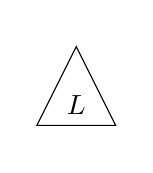
\begin{tikzpicture}
	\draw (0,0) node[anchor=north]{}
	-- (1,0) node[anchor=north]{}
	-- (.5,1) node[anchor=south]{}
	-- cycle;
	\draw (.5,.5) node[anchor=north]{$L$};
	\end{tikzpicture}}
\newcommand{\righttree}{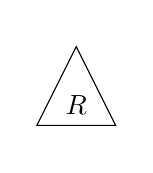
\begin{tikzpicture}
	\draw (0,0) node[anchor=north]{}
	-- (1,0) node[anchor=north]{}
	-- (.5,1) node[anchor=south]{}
	-- cycle;
	\draw (.5,.5) node[anchor=north]{$R$};
	\end{tikzpicture}}


\begin{document}	
	\title{Algorithmen und Datenstrukturen}
	\subtitle{Übung 9: AVL-Bäume \& Topologisches Sortieren}
	\author{Eric Kunze}
	\email{eric.kunze@tu-dresden.de}
	\city{TU Dresden}
%	\institute{Lehrstuhl für Grundlagen der Programmierung}
	\titlegraphic{\includegraphics[width=2cm]{../TUD-white.pdf}}
	\date{\formatdate{8}{12}{2021}}

	\maketitle


%%%%%%%%%%%%%%%%%%%%%%%%%%%%%%%%%%%%%%%%%%%%%%%%%%%%%%%%%%%%%%%%%%%%%%%%%%%%%


\begin{frame} \frametitle{Die nächsten Wochen}
	\begin{tabular}{lll}
		08.12.2021 & Übungsblatt 9 --- regulär \\
		\textbf{15.12.2021} & \textbf{keine Übung} \\
		22.12.2021 & Übungsblatt 10 \\
		\multicolumn{2}{l}{\hspace{3em}\textit{Weihnachten}} \\
		05.01.2022 & Übungsblatt 11
	\end{tabular}
\end{frame}

\section{AVL-Bäume}

\begin{frame} \frametitle{AVL-Bäume}
	Wir betrachten einen Baum $t$ und bezeichnen die \textit{Schlüssel} an den Knoten $n$ mit $s(n)$. 
	\pause
	
	\textbf{Suchbaum:} \Tree [.$s(n)$ [ .{\lefttree} ] [ .{\righttree} ] ] mit $L < s(n) < R$
	
	\pause
	
	Die \textbf{Höhe} des Baumes bezeichnen wir mit $h(t)$.
	Wir ordnen jedem Knoten $n$ einen \textbf{Balancefaktor} $b(n)$ zu:
	\begin{equation*}
		b(n) \defeq h(R) - h(L)
	\end{equation*}
	
	\pause
	\textbf{AVL-Baum:} Suchbaum mit $b(n) \in \menge{-1, 0, 1}$
\end{frame}

\begin{frame} \frametitle{Balancieren}
	\begin{itemize}
		\item Einfügen eines neuen Schlüssels $s$
		\item Berechne Balancefaktoren auf dem Pfad von $s$ zur Wurzel bis zum ersten Auftreten von $\pm 2$
		\pause
		\item \textbf{Balancierungsalgorithmus}: 
		\includegraphics[width=\linewidth]{./tut09_avl.jpg}
	\end{itemize}
\end{frame}

\begin{frame} \frametitle{Aufgabe 1}
	\textbf{Baum 1}:
	\begin{tabularx}{\linewidth}{m{2cm} m{.8cm} m{2cm} m{.8cm} m{2cm}}
		\begin{forest}
			[ $2$ [ $1$ ] [$3$ [,no edge, draw=none] [ $4$ ]  ] ] 
		\end{forest} 
		&
		$\overset{i(5)}{\longrightarrow}$
		&
		\begin{forest}
			[ $2^2$ [ $1$ ] [ $3^2$ [,no edge, draw=none] [ $4^1$ [,no edge, draw=none] [ $5^0$ ]  ] ]  ]
		\end{forest}  
		&
		$\overset{L(3)}{\longrightarrow}$
		&
		\begin{forest}
			[ $2$ [ $1$ ] [ $4$ [ $3$ ] [ $5$ ] ] ]
		\end{forest}
	\end{tabularx}
\end{frame}

\begin{frame} \frametitle{Aufgabe 1}
	\textbf{Baum 2}:
	
	\begin{tabularx}{\linewidth}{m{2cm} m{.8cm} m{4cm}}
		\begin{forest}
			[ $4$ [ $2$ [,no edge, draw=none] [ $3$ ]  ] [ $5$ ] ]
		\end{forest}
		&
		$\overset{i(1)}{\longrightarrow}$
		&
		\begin{forest}
			[ $4^{-1}$ [ $2^0$ [ $1^0$ ] [ $3$ ]  ] [ $5$ ] ]
		\end{forest} 
	\end{tabularx}
\end{frame}

\begin{frame} \frametitle{Aufgabe 1}
	\textbf{Baum 3}:
	\footnotesize
	\begin{tabularx}{\linewidth}{m{4cm} m{.5cm} m{2.8cm}}
		\begin{forest}
			[ $8$ [ $5$ [ $3$ [ $2$ ] [ $4$ ]] [ $7$ [ $6$ ] [,no edge, draw=none]  ] ] [ $10$ [ $9$ ] [ $11$ ] ] ]
		\end{forest}
		&
		$\overset{i(1)}{\longrightarrow}$
		&
		\begin{forest}
			[ $8^{-2}$ [ $5^{-1}$ [ $3^{-1}$ [ $2^{-1}$ [ $1^0$ ] [,no edge, draw=none]] [ $4$ ]] [ $7$ [ $6$ ] [,no edge, draw=none]  ] ] [ $10$ [ $9$ ] [ $11$ ] ] ]
		\end{forest} 
		\\
		&
		$\overset{R(8)}{\longrightarrow}$
		&
		\begin{forest}
			[ $5$ [ $3$ [ $2$ [ $1$ ] [,no edge, draw=none] ] [ $4$ ] ] [ $8$ [ $7$ [ $6$ ] [,no edge, draw=none]] [ $10$ [ $9$ ] [ $11$ ]] ] ]
		\end{forest} 
	\end{tabularx}
\end{frame}

\begin{frame} \frametitle{Aufgabe 1}
	\textbf{Baum 4}:
	\small
	\begin{tabularx}{\linewidth}{m{2cm} m{.5cm} m{2.5cm} m{.5cm} m{2cm}}
		\begin{forest}
			[ $5$ [ $2$ [ $1$ ] [ $4$ ] ] [ $6$ ] ]
		\end{forest} 
		&
		$\overset{i(3)}{\longrightarrow}$
		&
		\begin{forest}
			[ $5^{-2}$ [ $2^{1}$ [ $1$ ] [ $4^{-1}$ [ $3^0$ ] [,no edge, draw=none]] ] [ $6$ ] ]
		\end{forest} 
		&
		$\overset{L(2)}{\longrightarrow}$
		&
		\begin{forest}
			[ $5$ [ $4$ [ $2$ [ $1$ ] [ $3$ ] ] [,no edge, draw=none] ] [ $6$ ] ]
		\end{forest}  \\ \\
		& $\overset{R(5)}{\longrightarrow}$
		& 
		\begin{forest}
			[ $4$ [ $2$ [ $1$ ] [ $3$ ]] [ $5$ [,no edge, draw=none] [ $6$ ] ] ]
		\end{forest}
	\end{tabularx}
\end{frame}

\begin{frame}[fragile] \frametitle{Erinnerung: Bäume}
	\small
	\begin{lstlisting}[style=notebook]
typedef struct node *tree;
struct node { int key; tree left, right; };
	\end{lstlisting}

	\begin{minipage}{\dimexpr0.5\linewidth-\fboxrule-\fboxsep}
		\begin{tikzpicture}[%
			>=stealth',
			semithick,
			every node/.style={font=\scriptsize},
			inbox/.style={anchor=mid, font=\scriptsize, align=center, pos=0.5},
			]
			\draw[thick, rounded corners=2pt, color=cdpurple] (0,0) rectangle ++(2,1);
			\node[anchor=west, color=cdpurple] (struct node) at (2.05, 0.25) {\texttt{struct node}};
			\draw (0,0.5) -- (2,0.5)
			(1,0) -- (1,0.5);
			\path (0,0.5) rectangle ++(1,-0.5) node[inbox] (leftbox) {\texttt{left}} 
			rectangle ++(1, 0.5) node[inbox] (rightbox) {\texttt{right}}
			rectangle ++ (-2,0.5) node[inbox] {\texttt{key}};
			
			\draw[->, thick, color=cdblue] (1, 1.75) -- node[pos=0.2, right]{\texttt{tree t}} (1, 1);
			
			\draw[->, thick] (0.5,0) -- ++(-0.5,-0.75);
			\draw[->, thick] (1.5,0) -- ++( 0.5,-0.75);
			\node at (0,-1) {$\vdots$};
			\node at (2,-1) {$\vdots$};	
			
			\onslide<2->{%
				\draw[->, thick, color=cdgray] (0,1.75) --node[pos=0, above]{\texttt{tree* tp}} (1,1.75);
			}	
		\end{tikzpicture}
	\end{minipage}
	\onslide<3->{
	\begin{minipage}{\dimexpr0.5\linewidth-\fboxrule-\fboxsep}
		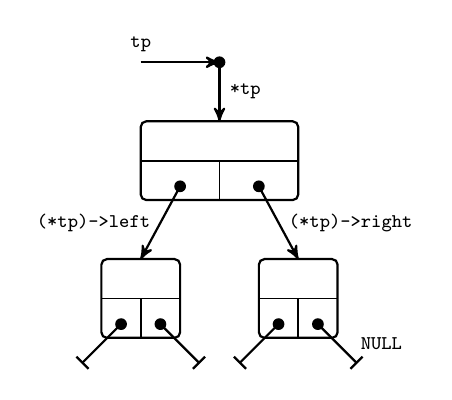
\begin{tikzpicture}[%
			>=stealth',
			semithick,
			every node/.style={font=\scriptsize},
			inbox/.style={anchor=mid, font=\scriptsize, align=center, pos=0.5},
			]
			\draw[thick, rounded corners=2pt] (0,0) rectangle ++(2,1);
			\draw (0,0.5) -- (2,0.5)
			(1,0) -- (1,0.5);
			\path (0,0.5) rectangle ++(1,-0.5) node[inbox] (leftbox) {} 
			rectangle ++(1, 0.5) node[inbox] (rightbox) {}
			rectangle ++ (-2,0.5) node[inbox] {};
			
			\draw[->, thick] (0,1.75) --node[pos=0, above]{\texttt{tp}} (1,1.75);
			\draw[->, thick] (1, 1.75) -- node[pos=0.5, right]{\texttt{*tp}} (1, 1);
			\node at (1,1.75) [circle,fill,inner sep=1.5pt] {};
			
			\node at (leftbox.center) [circle,fill,inner sep=1.5pt] {};
			\node at (rightbox.center) [circle,fill,inner sep=1.5pt] {};
			\draw[->, thick] (leftbox.center) --node[pos=0.5, left, anchor=east]{\texttt{(*tp)->left}} (0,-0.75);
			\draw[->, thick] (rightbox.center) --node[pos=0.5, right, anchor=west]{\texttt{(*tp)->right}} (2,-0.75);	
			
			% left child
			\draw[thick, rounded corners=2pt] (-0.5,-0.75) rectangle ++(1,-1);
			\draw (-0.5,-1.25) -- ++(1,0)
			(0,-1.25) -- ++(0,-0.5);
			\path (-0.5,-0.75) rectangle ++(1,-0.5) node[inbox] (kexbox2) {} 
			rectangle ++(-0.5, -0.5) node[inbox] (rightbox2) {}
			rectangle ++ (-0.5,0.5) node[inbox] (leftbox2) {};		
			
			\node at (leftbox2.center) [circle,fill,inner sep=1.5pt] {};
			\node at (rightbox2.center) [circle,fill,inner sep=1.5pt] {};
			\draw[-|, thick] (leftbox2.center) -- ++(-0.5,-0.5);
			\draw[-|, thick] (rightbox2.center) -- ++( 0.5,-0.5);
			
			% right child
			\draw[thick, rounded corners=2pt] (1.5,-0.75) rectangle ++(1,-1);
			\draw (1.5,-1.25) -- ++(1,0)
			(2,-1.25) -- ++(0,-0.5);
			\path (1.5,-0.75) rectangle ++(1,-0.5) node[inbox] (kexbox3) {} 
			rectangle ++(-0.5, -0.5) node[inbox] (rightbox3) {}
			rectangle ++ (-0.5,0.5) node[inbox] (leftbox3) {};		
			
			\node at (leftbox3.center) [circle,fill,inner sep=1.5pt] {};
			\node at (rightbox3.center) [circle,fill,inner sep=1.5pt] {};
			\draw[-|, thick] (leftbox3.center) -- ++(-0.5,-0.5);
			\draw[-|, thick] (rightbox3.center) -- ++( 0.5,-0.5) node[pos=0.5, anchor=west, right, inner sep=8pt]{\texttt{NULL}};
		\end{tikzpicture}
	\end{minipage}
	}
	\onslide<2->{%
		\begin{itemize}
			\item Verarbeitung eines Baumes: Einfachreferenzen (\texttt{tree t})
			\item Veränderung eines Baumes: Doppelreferenzen (\texttt{tree *tp})
		\end{itemize}%
	}
\end{frame}

\begin{frame}[fragile] \frametitle{Aufgabe 2 --- Teil (a)}
	\textbf{neuen Baum mit Balancefaktoren bestimmen}
	\begin{lstlisting}[style=notebook, basicstyle=\scriptsize\ttfamilywithbold]
int height(tree t) {
	if (t == NULL) return 0;
	
	int hl = height(t->left);
	int hr = height(t->right);
	return (hl > hr) ? hl + 1 : hr + 1;
}
	\end{lstlisting}
	\begin{lstlisting}[style=notebook, firstnumber=11, basicstyle=\scriptsize\ttfamilywithbold]
tree bfs(tree t) {
	if (t == NULL) return NULL;
		
	tree bf = malloc(sizeof(struct node));
	bf->key = height(t->right) - height(t->left);
	bf->left = bfs(t->left);
	bf->right = bfs(t->right);
	return bf;
}
	\end{lstlisting}
\end{frame}

\begin{frame}[fragile] \frametitle{Aufgabe 2 --- Teil (b)}
	\textbf{Linksrotation um die Wurzel}
	\begin{lstlisting}[style=notebook]
void lRot(tree *tp) {
	if (tp == NULL || *tp == NULL)
		return;
	
	tree rightChild = (*tp)->right;
	(*tp)->right = rightChild->left;
	rightChild->left = *tp;
	*tp = rightChild;
}
	\end{lstlisting}
	
\end{frame}

\section{Topologisches Sortieren}

\begin{frame} \frametitle{Topologisches Sortieren}
	\small
	\begin{itemize}
		\item Sortierung von \textit{Beziehungen} zwischen Objekten
		\item \textbf{Bsp.:} Ablauf eines Bauvorhabens \pause
		\begin{itemize}
			\item Baugrube ausheben (1) vor Fundament gießen (2)
			\item Fundament gießen (2) vor Wände setzen (3)
			\item $\dots$
			\item Elektrik im Bad (4) vor Fliesen (5)
			\item Wohnzimmer tapezieren (6) vor streichen (7)
			\item Fliesen (5) und Wände streichen (7) vor Möbel aufstellen (8)
		\end{itemize}
		\pause
		\begin{center}
			\scalebox{0.7}{
			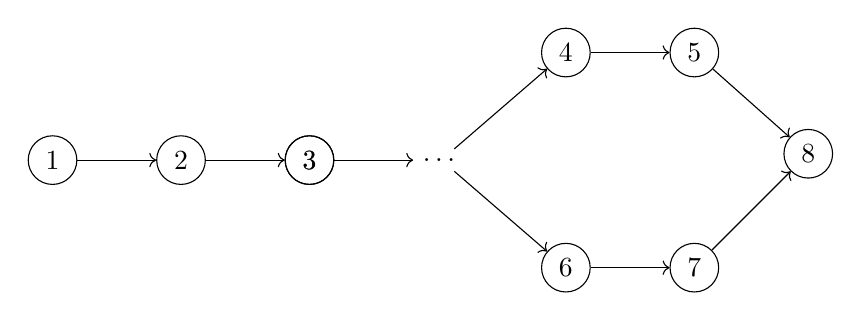
\begin{tikzpicture}
				\node [circle,draw] (1) {$1$};
				\node [circle,draw,right=of 1] (2) {$2$};
				\node [circle,draw,right=of 2] (3) {$3$};
				\node [circle,draw,right=of 2] (3) {$3$};
				\node [right=of 3] (dots) {$\dots$};
				\node [circle,draw,above right=of dots] (4) {$4$};
				\node [circle,draw,right=of 4] (5) {$5$};
				\node [circle,draw,below right=of dots] (6) {$6$};
				\node [circle,draw,right=of 6] (7) {$7$};
				\node [circle,draw,above right=of 7] (8) {$8$};
				
				% Kanten
				% \path (1) -> node[weight] {$3$} (3)
				\draw[->] (1) -> (2);
				\draw[->] (2) -> (3);
				\draw[->] (3) -> (dots);
				\draw[->] (dots) -> (4);
				\draw[->] (4) -> (5);
				\draw[->] (5) -> (8);
				\draw[->] (dots) -> (6);
				\draw[->] (6) -> (7);
				\draw[->] (7) -> (8);
			\end{tikzpicture}}
		\end{center}
		\pause
		\item In welcher Reihenfolge kann ich die Tätigkeiten abarbeiten?
	\end{itemize}
\end{frame}

\begin{frame} \frametitle{Topologisches Sortieren}
	\small
	Gegeben sei ein gerichteter, azyklischer Graph $G = (V,E)$. Eine \textbf{topologische Sortierung} von $G$ ist eine \textit{bijektive} Abbildung $\operatorname{ord} \colon V \to \menge{1, \dots, \card{V}}$, sodass für alle $v, v' \in V$ mit $(v,v') \in E$ die Relation
	$\operatorname{ord}(v) < \operatorname{ord}(v')$ gilt.
	
	\pause
	
	\textbf{Algorithmus:}
	
	\texttt{while} ( Elemente übrig ) \\
	\{  %\vspace{-\baselineskip}
		\begin{itemize}
			\item wähle Element $v$ ohne Vorgänger
			\item dekrementiere Anzahl der Vorgänger in den Nachfolgern von $v$
			\item füge $v$ der Ausgabeliste hinzu
			\item lösche $v$ aus $G$
		\end{itemize}
	\}
	 
\end{frame}

\begin{frame} \frametitle{Aufgabe 3}
	\textbf{Teil (a)}
	\begin{center}
		\scalebox{1}{
		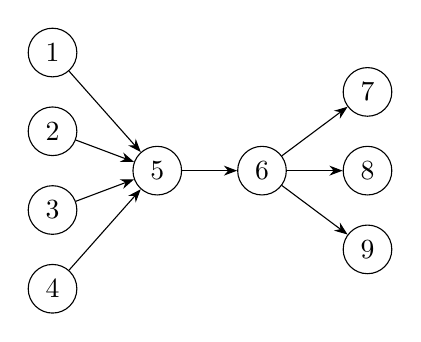
\begin{tikzpicture}		
			\node [circle,draw] (1) at (0,1.5)  {$1$};
			\node [circle,draw] (2) at (0,0.5)  {$2$};
			\node [circle,draw] (3) at (0,-0.5) {$3$};
			\node [circle,draw] (4) at (0,-1.5) {$4$};
			
			\node [circle,draw] (5) at (1.33,0)  {$5$};
			\node [circle,draw] (6) at (2.66,0)  {$6$};
			
			\node [circle,draw] (7) at (4,1)  {$7$};
			\node [circle,draw] (8) at (4,0)  {$8$};
			\node [circle,draw] (9) at (4,-1) {$9$};
			
			% Kanten
			% \path (1) -> node[weight] {$3$} (3)
			\draw[->, arrows=-Stealth] (1) -> (5);
			\draw[->, arrows=-Stealth] (2) -> (5);
			\draw[->, arrows=-Stealth] (3) -> (5);
			\draw[->, arrows=-Stealth] (4) -> (5);
			\draw[->, arrows=-Stealth] (5) -> (6);
			\draw[->, arrows=-Stealth] (6) -> (7);
			\draw[->, arrows=-Stealth] (6) -> (8);
			\draw[->, arrows=-Stealth] (6) -> (9);
		\end{tikzpicture}}
	\end{center}
	\pause
	Es gibt $4! \cdot 1! \cdot 3! = 24 \cdot 1 \cdot 6 = 144$ viele topologische Sortierungen.
\end{frame}

\begin{frame} \frametitle{Aufgabe 3}
	\textbf{Teil (b)}
	
	Es werden alle Möglichkeiten mit der $1$ am Anfang gestrichen, d.h. im ersten Block gibt es nur noch $4! - 3! = 24 - 6$ viele Möglichkeiten --- insgesamt also 
	\begin{equation*}
		(4! - 3!) \cdot 1! \cdot 3! = 18 \cdot 1 \cdot 6 = 108 \, .
	\end{equation*}

	\pause
	
	\textbf{Teil (c)}
	\begin{center}
		\scalebox{1}{
		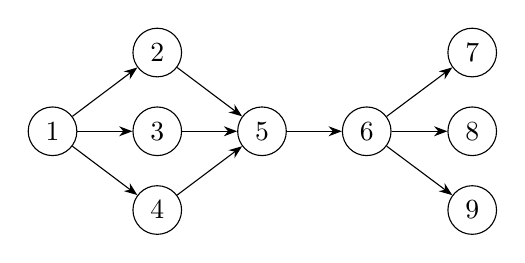
\begin{tikzpicture}		
			\node [circle,draw] (1) at (-1.33,0)  {$1$};
			\node [circle,draw] (2) at (0,1)  {$2$};
			\node [circle,draw] (3) at (0,0) {$3$};
			\node [circle,draw] (4) at (0,-1) {$4$};
			
			\node [circle,draw] (5) at (1.33,0)  {$5$};
			\node [circle,draw] (6) at (2.66,0)  {$6$};
			
			\node [circle,draw] (7) at (4,1)  {$7$};
			\node [circle,draw] (8) at (4,0)  {$8$};
			\node [circle,draw] (9) at (4,-1) {$9$};
			
			% Kanten
			% \path (1) -> node[weight] {$3$} (3)
			\draw[->, arrows=-Stealth] (1) -> (2);
			\draw[->, arrows=-Stealth] (1) -> (3);
			\draw[->, arrows=-Stealth] (1) -> (4);
			
			\draw[->, arrows=-Stealth] (2) -> (5);
			\draw[->, arrows=-Stealth] (3) -> (5);
			\draw[->, arrows=-Stealth] (4) -> (5);
			\draw[->, arrows=-Stealth] (5) -> (6);
			\draw[->, arrows=-Stealth] (6) -> (7);
			\draw[->, arrows=-Stealth] (6) -> (8);
			\draw[->, arrows=-Stealth] (6) -> (9);
		\end{tikzpicture}}
	\end{center}
\end{frame}

\end{document}